\chapter{verwandte Arbeiten}
\label{relatedWork}

Da GraphQL eine stetig wachsende Beliebtheit verzeichnet \cite{graphql-growing-report}[vgl. Language Features] steigt auch der Bedarf und das Interesse an Testmethoden.
Aktuell gibt es für GraphQL noch eine Lücke an produktionsreifen Testtools, insbesondere automatischen Testtools.
Eine wachsende Anzahl an Forschungsprototypen beziehungsweise untersuchten Methoden ist allerdings zu verzeichnen.
In diesem Kapitel sollen diese Methoden benannt werden und Verwandheiten, Unterschiede oder thematische Überschnitte von dieser und anderen Arbeiten benannt werden.

\section{Property Based Testing}

In \textit{Automatic Property-based Testing of GraphQL APIs}~\cite{property-based-testing} wird der Ansatz des Property-based Testing verfolgt, um Integrationstests zu erstellen.
Property-based Testing ist laut dem Paper heute Synonym mit "Random Testing"\cite{property-based-testing}[vgl. 2B] wobei zufällig hierbei meint, dass die Eingabedaten und Routen zufällig generiert werden.
Wie zuvor erwähnt soll diese Arbeit als Motivation für unsere zu entwickelnde Methode dienen, indem wir versuchen eine bessere Graphabdeckung zu erreichen als durch
das Zufällige Testen welches einige Limitierungen aufweist.
Wir wollen hier das \textit{Property-based Testing} noch einmal untersuchen und die Probleme konkreter aufzeigen.
Der allgemeine Funktionsablauf der Testgenerierung laut Paper ist wie folgt:

\begin{center}
    \begin{itemize}
        \item[1.] Vom Schema, generiere Typ-Spezifikationen
        \item[2.] Generiere einen Generator der zufällig eine Liste an Query-Objekten erstellen kann
        \item[3.] Generiere n Querys
        \item[4.] Transformiere die Queries in GraphQL-Format
        \item[5.] Führe die Queries auf dem SUT (system under test) aus
        \item[6.] Evaluiere die Ergebnisse auf ihre Properties
    \end{itemize}{\cite[vgl. 3. Proposed Method]{property-based-testing}}
\end{center}

Punkt 2 wird der Hauptunterscheidungspunkt beider Arbeiten sein, denn hier sind dann zwei gänzlich unterschiedliche Konzepte umgesetzt
Dieser ist beim Property-Based Testing,nämlich ein Query-Generator der mithilfe der Clojure-Bilbiothek Serene\cite{clojureserene}
Clojure.Specs\cite{clojurespec} generiert und diese Clojure.Specs\cite{clojurespec} dann nutzt, um mit der Clojure-Bilbiothek Malli\cite{clojuremalli} dann Daten für die Testqueries zu generieren.
Betrachtet man die Arbeit aus einer graphentheoretischen Sicht, so zeigt sich, dass das Property-based Testing auf Graphstrukturen arbeitet, diese allerdings in seiner eigenen Verarbeitung nicht umsetzt.
Unsere herangehensweise wird sich hiervon gänzlich unterscheiden.
Im Sinne vom Property-based Testing ist diese Herangehensweise allerdings sehr sinnvoll gewesen da Malli\cite{clojuremalli} de-facto Standard für Property-based Testing in der Clojure-Welt ist.
Hauptbeitrag der Arbeit war, einen Generator für Malli zu schreiben der in der Lage ist GraphQL-Querys zu generieren.
Geht man jedoch davon aus, dass das Ziel eine ideale Überdeckung des Graphens jeder größe und jeder Struktur ist, so
ist diese herangehensweise nicht die beste.\cite{property-based-testing}[vgl. 3C]
Dies folgt, da die benutzte Bibliothek Malli eben keine Pfade als solches kennt, sondern nur zufällige Nachfolger eines Typens.
Daher wird ein Rekursionslimit zwingend benötigt weil es anders nicht möglich ist Zyklen in der Abhängigkeit der Typen aufzulösen.
Laut dem Paper gilt \textit{ein größeres und mehr rekursives (GraphQL)-Schema würde nicht skalieren und der (zufällig) iterative Ansatz ist besser als eine Breitensuche}~\cite{property-based-testing}[vgl. 3C].
Diese Behauptung betrachten wir als falsch und behaupten, dass es besser möglich ist.
Dies zu zeigen bleibt Gegenstand der folgenden Arbeit.


\section{heuristisch suchen basiertes Testen}

EvoMaster\cite{evo-master} ist ein Open-Source Tool welches sich automatisiertes Testen von Rest-APIs und GraphQL APIs zur Aufgabe gemacht hat.
Aktuell kann durch EvoMaster sowohl WhiteBox Testing als auch BlackBox Testing durchgeführt werden jedoch ist ein
Whitebox Test mittels Vanilla-EvoMaster nur für Rest-APIs möglich die mit der JVM lauffähig sind.
Im Paper \textit{White-Box and Black-Box Fuzzing for GraphQL APIs}~\cite{belhadi2022whitebox} wurde eine Erweiterung für EvoMaster
erstellt welches GraphQL Tests generieren kann.
Hierbei soll sowohl WhiteBox als auch BlackBox Testing möglich sein.
Das erstellte Framework in diesem Paper arbeitet nach dem Prinzip das in Abbildung~\ref{evomast} dargestellt ist.

\begin{figure}
    \centering
    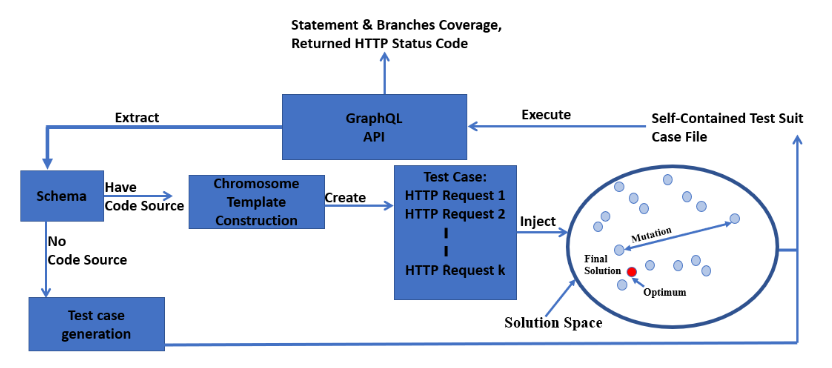
\includegraphics[width=\textwidth,height=\textheight,keepaspectratio]{content/hauptteil/relatedWork/evomaster_framework}
    \caption{Arbeitsweise EvoMaster}
    \label{evomast}
\end{figure}

WhiteBox Testing ist möglich insofern Zugang zum GraphQL-Schema und zum Source Code der API gegeben ist.
Andernfalls ist nur BlackBox Testing möglich.
Zur Testgenerierung wird ein genetischer Algorithmus genutzt welcher die Tests generiert.
Ein genetischer Algorithmus ist ein Optimierungsalgorithmus der von der natürlichen Evolution inspiriert ist.
Dabei werden verschiedene Lösungen eines Problems in Generationen erstellt, verändert und nach bestimmten Bedingungen ausgewählt,
sodass das gewünschte Ergebnis stetig besser wird~\cite[vgl.]{genalgo}.
Während ein genetischer Algorithmus sich einer Lösung annähert, berechnet er diese jedoch nicht zuverlässig ideal~\cite[vgl. Fazit]{genalgo}.
Im Gegensatz dazu ist der Ansatz dieser Arbeit ein iterativer Algorithmus der eine ideale Lösung im ersten Durchlauf erreicht.
Die ideale Lösung bezieht sich hierbei auf ein Abdeckungskriterium, dass die Testpfade erfüllen müssen, die durch unseren Algorithmus erfüllt werden.
Ein genetischer Algorithmus kann das Abdeckungskriterium irgendwann auch erfüllen jedoch kann keine allgemeine Aussage darüber gemacht werden, wann er dieses erreicht.
Während die BlackBox-Tests mit ähnlichen Hürden zu kämpfen haben wie das \textit{Property-based Testing} zeigt sich, dass ein WhiteBox
Ansatz eine Verbesserung bringen kann - allerdings muss starkes Domänenwissen in den Suchalgorithmus eingearbeitet werden, sodass man noch fern
von einer WhiteBox-Testautomatisierung ist~\cite[vgl. Discussion and Future Directions]{belhadi2022whitebox}.

\section{Deviation Testing}

Da GraphQL dynamisch auf Anfragen reagiert und es somit möglich ist, in seiner Anfrage einzelne Felder mit einzubeziehen
oder auch auszuschließen ist dies im Grunde genommen ein einzelner Testfall.
Im Paper \textit{Deviation Testing: A Test Case Generation Technique for GraphQL APIs}~\cite{deviation} wird diese Gegebenheit benutzt und
aus einer selbstdefinierten Query werden verschiedene Variationen erzeugt~\cite[vgl. 3]{deviation}.
Da Deviation Testing jedoch nur bestehende Tests erweitert um mögliche Felder mitzutesten werden hier keine neuen Tests  im Sinne der Pfadabdeckung generiert.
Durch Deviation Testing werden bestehende Tests nur erweitert.
Die durch Variation erstellten Tests stellen jeweils stets immer den gleichen Pfad im Graphen dar und nur die Auswahl der verschiedenen $SCALAR$ Felder wird verändert.
Somit kann Deviation Testing maximal dazu dienen, die Codeabdeckung eines einzelnen Pfades zu maximieren jedoch nicht die Graphabdeckung insgesamt zu erhöhen.

\section{Query Harvesting}

Klassisches Testen von Anwendungen beeinhaltet, dass nach Möglichkeit das komplette System getestet wird bevor es verwendet wird.
Im Paper \textit{Harvesting Production GraphQL Queries to Detect Schema Faults}~\cite{harvesting} wird ein gänzlich anderer Ansatz verfolgt.
Hierbei ist es nicht wichtig, dass die gesamte GraphQL-API vor der Veröffentlichung getestet ist, sondern echte Queries die in Produktion ausgeführt wurden zu sammeln.
Der Ansatz, der hierbei verfolgt wird, begründet sich so, dass ein Testraum für GraphQL potenziell unendlich sein kann und es sehr wahrscheinlich ist, dass nur ein kleiner
Teil der API wirklich intensiv genutzt wird, sodass auch nur dieser Teil wirklich stark durch Tests abgedeckt werden muss.
Der vorgestellte Prototyp AutoGraphQL läuft hierbei in zwei Phasen wobei in der ersten Phase alle einzigartigen Anfragen gesammelt werden.
In der zweiten Phase werden dann aus den gesammelt Anfragen Tests generiert.
Dabei wird für jede gesammelte Anfraege genau ein Test-Case erstellt.
Bei dieser Art des Testens wird insbesondere darauf Wert gelegt, dass Veränderungen im GraphQL-Schema zu keinem Fehler führen.
Während in dieser Arbeit überprüft wird, dass Querys im laufenden Produktlebenszyklus nicht zu einem Fehler führen, wird außer Acht gelassen,
dass eine Query korrekt für AutoGraphQL sein kann aber trotzdem falsch, indem zum Beispiel falsche Daten zurückgegeben werden
durch falsche Referenzierung oder ähnlichem.
Somit eignet sich AutoGraphQL vor allem als Monitoring-Software, die gleichzeitig dafür sorgt, dass die Integrität der GraphQL-API bei Veränderungen
testbar ist.

\section{Vergleich der Arbeiten}
Folgender Vergleich soll die eben vorgestellten Arbeiten noch einmal kurz einordnen.
\begin{center}
    \begin{table}[!hbt]
        \begin{tabularx}{\textwidth}{|C|C|C|C|C|C|}
            \hline
            \textbf{ Arbeit / Kriterium} & \textbf{Property Based Testing} & \textbf{heuristisch suchenbasiertes Testen} & \textbf{Deviation-Testing} & \textbf{Query Harvesting} \\
            \hline
            Generierungsart & Zufallsbasierte Routengenerierung & Heuristische Suche & Erweiterung von bestehenden Tests & Sammeln von Querys und daraus Tests generieren \\
            \hline
            Überdeckung & Zufällig, stark abhängig von Schema  & abhängig ob Zugang zu Source Code, Zufällig aber optimaler & stark abhängig von selbst geschriebenen Tests  & stark Abhängig von Nutzeranfragen \\
            \hline
            Orakel & simples Raten & mit Source Code: Analyse & Aus entwickelten Tests &  Aus gestellten Querys \\
            \hline
            Ausführzeit & vor Produktion & vor Produktion & vor Produktion & Verifikation / Wartung \\
            \hline
            Use-Case & allgemeines Testen & allgemeines Testen & allgemeines Testen & Testen bei Code-Änderung \\
            \hline
        \end{tabularx}
        \caption{Vergleich der verwandten Arbeiten}
    \end{table}
\end{center}


